%! suppress = MissingImport
Figure~\ref{fig:templates} is a set of four templates for the Cow Pi circuit (one for each combination of pushbuttons (2-lead or 4-prong) and slide-switches (2-pin or 3-pin).
Each dot (\tikz{\draw[white,fill=gray] (0,0) +(0,3pt) circle (1pt);}) represents a breadboard contact point.
Each dot with a circle (\tikz{\drawtarget{0}{3pt} \draw[white,fill=gray] (0,0) +(0,3pt) circle (1pt);}) is a contact point in which you will insert a jumper lead.
Attached to most of these circles is the contact point for the other end of the jumper wire (\tikz{\drawlabelledtarget{0}{0}{1}{k64} \draw[white,fill=gray] (0,0) circle (1pt);}).
The footprints of several components are shown as light-gray outlines;
resistors (\tikz{\ctikzset{bipoles/resistor/height=0.2}\ctikzset{bipoles/resistor/width=0.3}\draw (0,0) to[R] (1,0)}) and LEDs (\tikz{\ctikzset{bipoles/diode/height=0.2}\ctikzset{bipoles/diode/width=0.2}\draw (0,0) to[led] (1,0)}) are shown using their conventional symbols.
Squares (\tikz{\draw[white,fill=gray] (0,0) +(2pt,3pt) circle (1pt); \draw (0,0) +(0,1pt) rectangle +(4pt,5pt);}) are where you'll insert component individual pins,
and rectangles (\tikz{\draw (0,0) +(0,1pt) rectangle +(11pt,5pt); \draw[white,fill=gray] (0,0) +(2pt,3pt) circle (1pt); \draw[white,fill=gray] (0,0) +(5.5pt,3pt) circle (1pt); \draw[white,fill=gray] (0,0) +(9pt,3pt) circle (1pt);}) are where you'll insert components' in-line pins.
Finally, the four corners (\tikz{\draw[white,fill=gray] (0,0) +(2pt,3pt) circle (1pt); \draw (0,1pt) -- (4pt,5pt); \draw (0,5pt) -- (4pt,1pt);}) are used to align the template on your solderless breadboard.

%TODO: add dip1 switch subfigures
\begin{figure}[p]
    \subfloat[Template that uses 3-pin slide-switches and 2-lead pushbuttons.]{
        \hspace{-.5in}
        \begin{tikzpicture}[x=.1in, y=.1in]
            \drawbreadboard
            \drawnano{1}{3}{Arduino Nano}
            \drawledcircuit
            \drawnand{18}{5}
            \drawswitches{\controlsstartat+1}
            \drawbuttons{\controlsstartat+11}{2}
            \drawkeypadandtargets{\controlsstartat}
            \drawdisplay{48}
        \end{tikzpicture}
    }
    \vspace{.5in}
    \subfloat[Template that uses 3-pin slide-switches 4-prong pushbuttons.]{
        \hspace{-.5in}
        \begin{tikzpicture}[x=.1in, y=.1in]
            \drawbreadboard
            \drawnano{\mcux}{\mcuy}{Arduino Nano}
            \drawledcircuit
            \drawnand{\nandx}{\nandy}
            \drawswitches{\controlsstartat+1}
            \drawbuttons{\controlsstartat+11}{4}
            \drawkeypadandtargets{\controlsstartat}
            \drawdisplay{48}
        \end{tikzpicture}
    }
    \caption{Templates to improve accuracy when constructing the Cow Pi circuit on a solderless breadboard.}\label{fig:templates}%\addcontentsline{toc}{section}{Breadboard Templates}
\end{figure}

\textit{Optionally}, print the page that has the template appropriate to your particular switches and pushbuttons.
When (if) you do so, be sure to select ``Actual size'' (see Figure~\ref{fig:printmenu}).
If you mistakenly select a different option, the template will not line up properly with your breadboard: even a tiny scaling factor will add-up over the length of the breadboard.
Using the lead from a jumper wire, punch holes into the four $\times$s at the corners (contact points a1, j1, a63, and j32); see Figure~\ref{fig:punchingholes}.
Place the lead from a jumper wire into each of the four holes, and insert the leads into the corresponding contact points on the breadboard, pinning the template to the breadboard.
Confirm that the four jumpers are aligning the template to the breadboard by visually checking that the four leads are in the breadboard's contact points a1, j1, a63, and j32 (see Figure~\ref{fig:confirmalignment}).

\begin{figure}
    \centering
    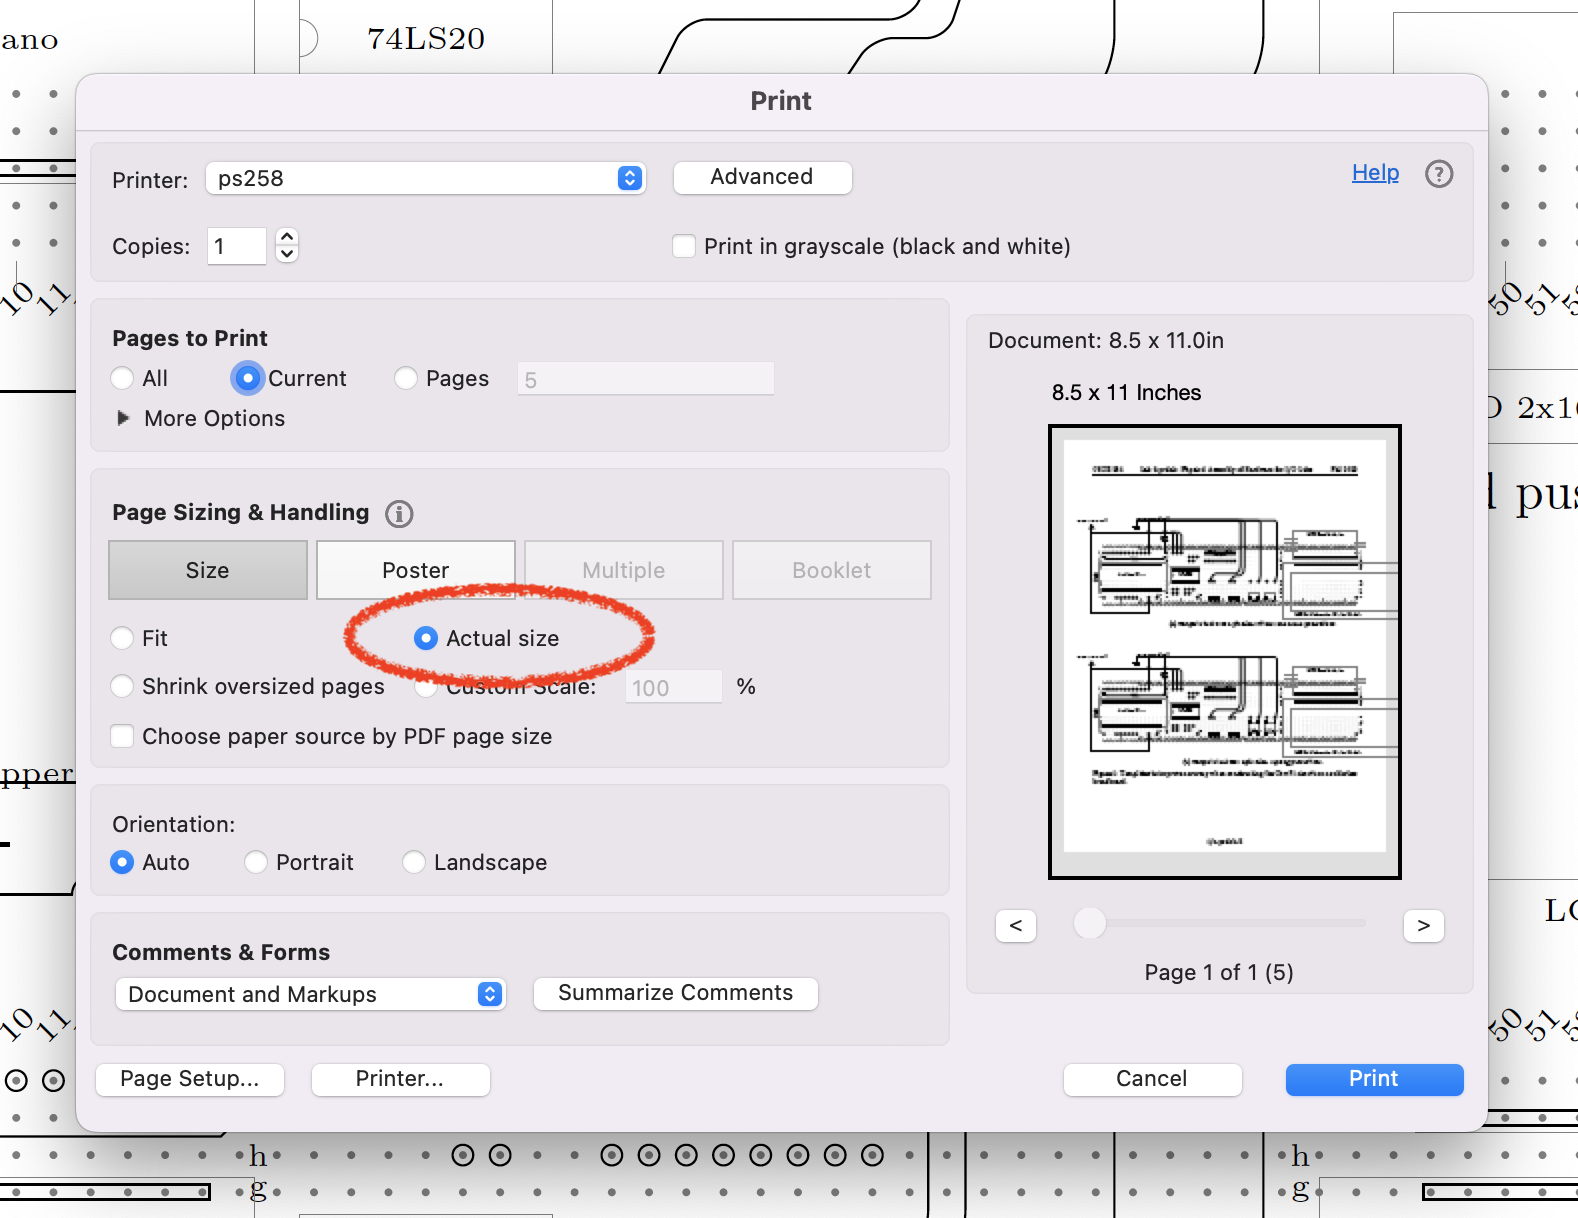
\includegraphics[width=0.5\textwidth]{breadboard-guides/print-menu}
    \caption{When printing a breadboard template, be sure to select ``Actual size''.} \label{fig:printmenu}
\end{figure}

\begin{figure}
    \centering
    \subfloat[Punching alignment holes in breadboard template.]{
        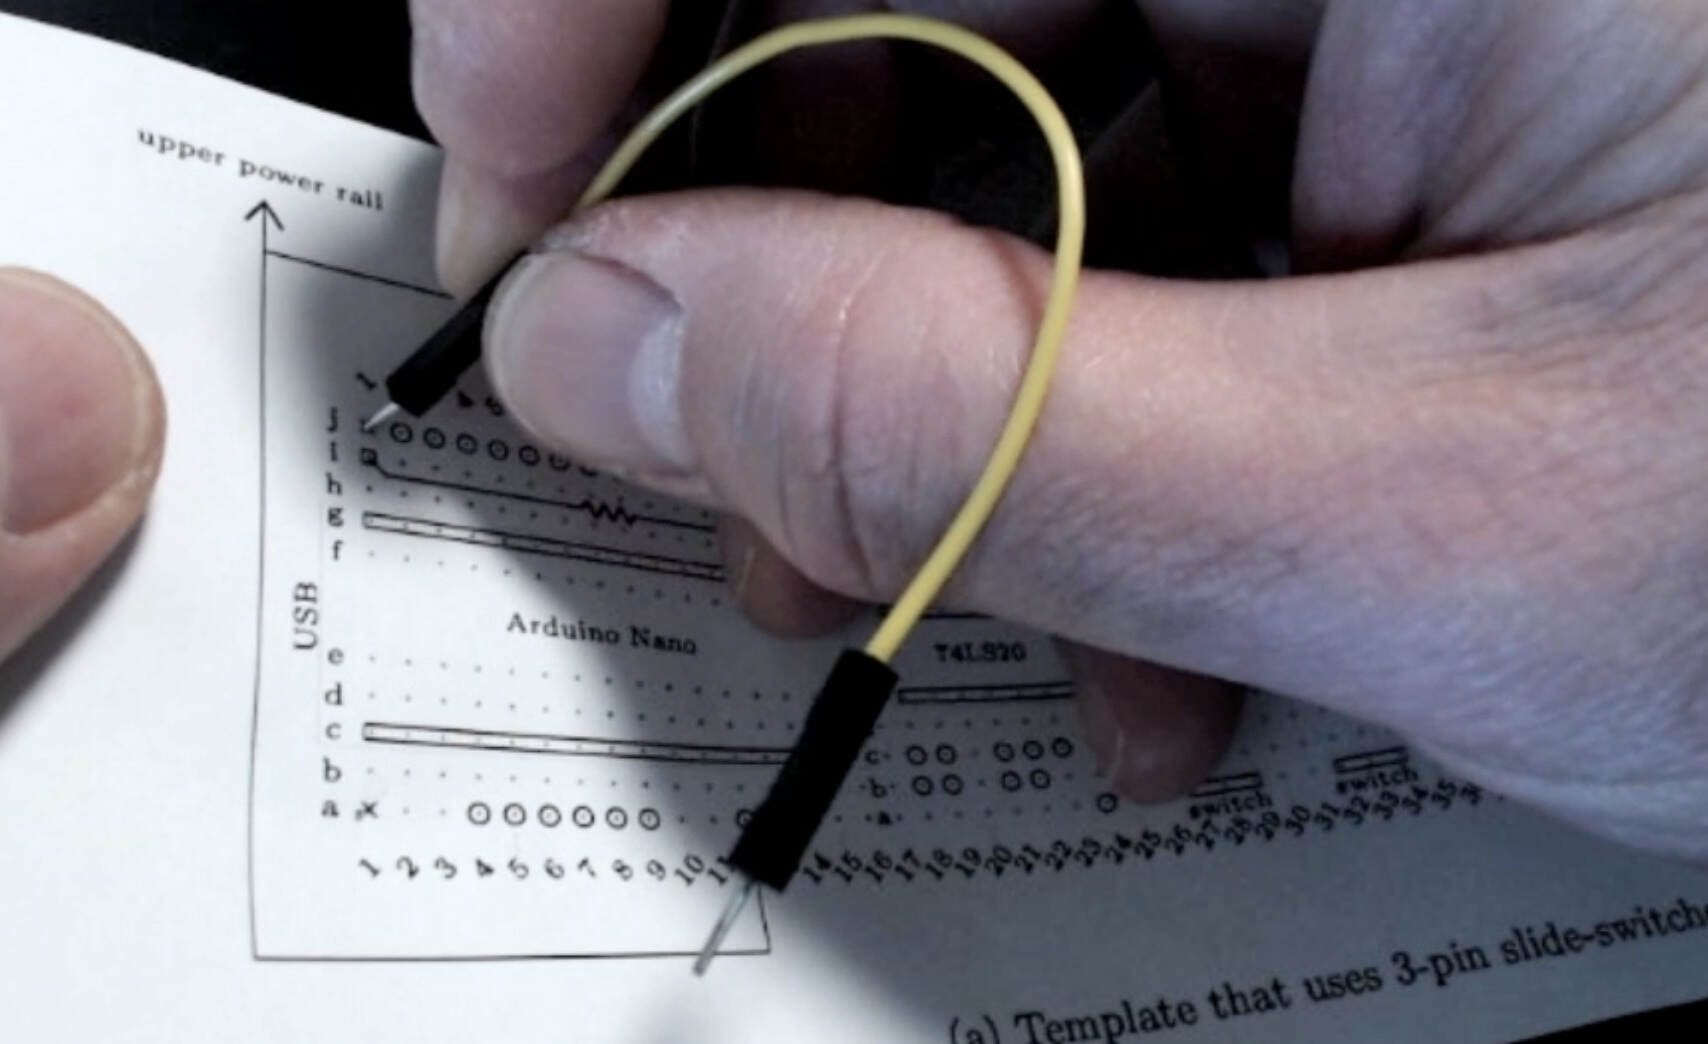
\includegraphics[height=3cm]{breadboard-guides/punching-holes}
        \label{fig:punchingholes}
    }
    \hfil
    \subfloat[Confirming that the corners of the template are aligned with the corners of the breadboard.]{
        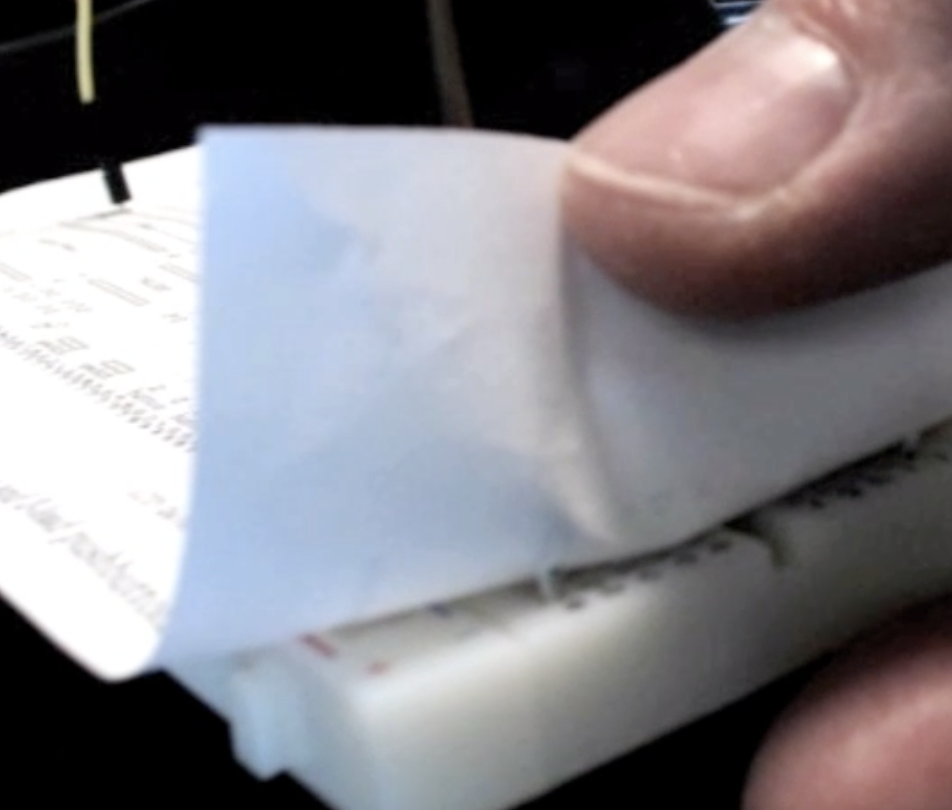
\includegraphics[height=3cm]{breadboard-guides/confirm-alignment}
        \label{fig:confirmalignment}
    }
    \caption{Preparing a breadboard template.}
\end{figure}

